% Pengaturan ukuran teks dan bentuk halaman dua sisi
\documentclass[12pt]{report}

% Pengaturan ukuran halaman dan margin
\usepackage[a4paper,top=30mm,left=30mm,right=20mm,bottom=25mm]{geometry}

% Pengaturan ukuran spasi
\usepackage[singlespacing]{setspace}

% Pengaturan caption untuk tabel
\usepackage{caption}

% Judul dokumen
\title{Proposal Tugas Akhir ITS}
\author{Musk, Elon Reeve}

% Pengaturan detail pada file PDF
\usepackage[pdfauthor={\@author},bookmarksnumbered,pdfborder={0 0 0}]{hyperref}


% Pengaturan ukuran indentasi
\setlength{\parindent}{2em}

% Package lainnya
\usepackage{changepage}
\usepackage{etoolbox} % Mengubah fungsi default

% Pengaturan jenis karakter
\usepackage[utf8]{inputenc}

\usepackage[style=apa, backend=biber]{biblatex}
\usepackage{enumitem} % Pembuatan list
\usepackage{lipsum} % Pembuatan template kalimat
\usepackage{graphicx} % Input gambar
\usepackage{longtable} % Pembuatan tabel
\usepackage[table,xcdraw]{xcolor} % Pewarnaan tabel
\usepackage{eso-pic} % Untuk menggunakan background image di halaman
\usepackage{txfonts} % Font times
\usepackage{changepage} % Pembuatan teks kolom
\usepackage{multicol} % Pembuatan kolom ganda
\usepackage{multirow} % Pembuatan baris ganda
\usepackage{tabularx} % Untuk mengatur kolom, seperti grid pada CSS
\usepackage{wrapfig}

% Pengaturan format daftar isi, daftar gambar, dan daftar tabel
\usepackage{tocloft}
\setlength{\cftsecindent}{0cm}
\setlength{\cftsubsecindent}{2em}
\setlength{\cftbeforechapskip}{1.5ex}
\setlength{\cftbeforesecskip}{1.5ex}
\setlength{\cftbeforetoctitleskip}{0cm}
\setlength{\cftbeforeloftitleskip}{0cm}
\setlength{\cftbeforelottitleskip}{0cm}
\renewcommand{\cftsecfont}{\normalfont\bfseries}% membuat judul section pada daftar isi menjadi bold
\renewcommand{\cftsecpagefont}{\normalfont\bfseries}% membuat nomor section daftar isi menjadi bold
\renewcommand{\cfttoctitlefont}{\hfill\Large\bfseries} % command untuk membuat heading bold dan besar
\renewcommand{\cftaftertoctitle}{\hfill}
\renewcommand{\cftloftitlefont}{\hfill\Large\bfseries}
\renewcommand{\cftafterloftitle}{\hfill}
\renewcommand{\cftlottitlefont}{\hfill\Large\bfseries}
\renewcommand{\cftafterlottitle}{\hfill}

% Definisi untuk "Hati ini sengaja dikosongkan"
\patchcmd{\cleardoublepage}{\hbox{}}{
	\thispagestyle{empty}
	\vspace*{\fill}
	\begin{center}\textit{[Halaman ini sengaja dikosongkan]}\end{center}
	\vfill}{}{}

% Pengaturan penomoran halaman
\usepackage{fancyhdr}
\fancyhf{}
\renewcommand{\headrulewidth}{0pt}
\pagestyle{fancy}
\fancyfoot[C,CO]{\thepage}
\patchcmd{\chapter}{plain}{fancy}{}{}
\patchcmd{\chapter}{empty}{plain}{}{}

% Pengaturan format judul bab
\usepackage{titlesec}
\renewcommand{\thesection}{\arabic{section}}
\titleformat{\chapter}[display]{\bfseries\Large}{BAB \centering\Roman{chapter}}{0ex}{\vspace{0ex}\centering}
\titleformat*{\section}{\large\bfseries}
\titleformat*{\subsection}{\normalsize\bfseries}
\titlespacing{\section}{0ex}{3ex}{1.5ex}
\titlespacing{\subsection}{0ex}{3ex}{1.5ex}
\titlespacing{\subsubsection}{0ex}{0.5ex}{0ex}
\setcounter{secnumdepth}{3} % Untuk memberi penomoran pada \subsubsection

\counterwithin{figure}{section}
\counterwithin{table}{section}

% Mengganti figure dan table menjadi gambar dan tabel
\renewcommand{\figurename}{Gambar}
\renewcommand{\tablename}{Tabel}

% Tambahkan format tanda hubung yang benar di sini
\hyphenation{
  ro-ket
  me-ngem-bang-kan
  per-hi-tu-ngan
}

% Menambahkan resource daftar pustaka
\addbibresource{pustaka/pustaka.bib}

% Isi keseluruhan dokumen
\begin{document}

  % Nomor halaman pembuka dimulai dari sini
  \pagenumbering{roman}

  % Atur ulang penomoran halaman
  \setcounter{page}{1}

  % Sampul Bahasa Indonesia
  \newcommand\covercontents{sampul/konten-id.tex}
  \input{sampul/sampul-luar.tex}

  % Sampul Bahasa Inggris
  \renewcommand\covercontents{sampul/konten-en.tex}
  \input{sampul/sampul-luar.tex}

  % Lembar pengesahan
  \begin{center}
	\large
  \textbf{LEMBAR PENGESAHAN}
\end{center}

% Menyembunyikan nomor halaman
\thispagestyle{empty}

\begin{center}
  % Ubah kalimat berikut dengan judul tugas akhir
  \textbf{PENGEMBANGAN ANEMOMETER ULTRASONIC DALAM RUANGAN
  	BERBASIS RASPBERRY PI PICO}
\end{center}

\begingroup
  % Pemilihan font ukuran small
  \small

  \begin{center}
    % Ubah kalimat berikut dengan pernyataan untuk lembar pengesahan
    \textbf{PROPOSAL TUGAS AKHIR} \\
    Diajukan untuk memenuhi salah satu syarat memperoleh gelar
    Sarjana Teknik pada 
    Program Studi S-1 Teknik Komputer \\
    Departemen Teknik Komputer \\
    Fakultas Teknologi Elektro dan Informatika Cerdas \\
    Institut Teknologi Sepuluh Nopember
  \end{center}

  \begin{center}
    % Ubah kalimat berikut dengan nama dan NRP mahasiswa
    Oleh: \textbf{Ghiyas Ash-Shidiqie Rismawan} \\
    NRP. 0721 19 4000 0014
  \end{center}

  \begin{center}
    Disetujui oleh Tim Penguji Proposal Tugas Akhir:
  \end{center}

  \begingroup
    % Menghilangkan padding
    \setlength{\tabcolsep}{0pt}

    \noindent
    \begin{tabularx}{\textwidth}{X c}
      % Ubah kalimat-kalimat berikut dengan nama dan NIP dosen pembimbing pertama
      Dion Hayu Fandiantoro, S.T., M.Eng.          & (Pembimbing) \\
      NIP: 19680601199512 1 009       & \\
      &  \\
      &  \\
      % Ubah kalimat-kalimat berikut dengan nama dan NIP dosen pembimbing kedua
      Arief Kurniawan, S.T, M.T.     & (Ko-Pembimbing) \\
      NIP: 19740907200212 1 001        & \\
      &  \\
      &  \\
      % Ubah kalimat-kalimat berikut dengan nama dan NIP dosen penguji pertama
      (...)  & (Penguji I) \\
      NIP: ...        & \\
      &  \\
      &  \\
      % Ubah kalimat-kalimat berikut dengan nama dan NIP dosen penguji kedua
      (...)  & (Penguji II) \\
      NIP: (...)        & \\
      &  \\
      &  \\
      % Ubah kalimat-kalimat berikut dengan nama dan NIP dosen penguji ketiga
      (...)             & (Penguji III) \\
      NIP: (...)        & \\
    \end{tabularx}
  \endgroup

  \vspace{4ex}

  \begin{center}
    % Ubah text dibawah menjadi tempat dan tanggal
    \textbf{SURABAYA} \\
    \textbf{Desember, 2022}
  \end{center}
\endgroup

  \newpage

  % Lembar pengesahan
  \begin{center}
	\large
  \textbf{APPROVAL SHEET}
\end{center}

% Menyembunyikan nomor halaman
\thispagestyle{empty}

\begin{center}
  % Ubah kalimat berikut dengan judul tugas akhir
  \textbf{DEVELOPMENT OF INDOOR ULTRASONIC ANEMOMETER BASED ON RASPBERRY PI PICO}
\end{center}

\begingroup
  % Pemilihan font ukuran small
  \small

  \begin{center}
    % Ubah kalimat berikut dengan pernyataan untuk lembar pengesahan
    \textbf{FINAL PROJECT PROPOSAL} \\
    Submitted to fulfill one of the requirements for obtaining a degree
    Bachelor of Engineering at 
    Undergraduate Study Program of Computer Engineering \\
    Department of Computer Engineering \\
    Faculty of Intellegent Electrical and Informatics Technology \\
    Sepuluh Nopember Institute of Technology
  \end{center}

  \begin{center}
    % Ubah kalimat berikut dengan nama dan NRP mahasiswa
    By: \textbf{Ghiyas Ash-Shidiqie Rismawan} \\
    NRP. 0721 19 4000 0014
  \end{center}

  \begin{center}
    Approved by Final Project Proposal Examiner Team:
  \end{center}

  \begingroup
    % Menghilangkan padding
    \setlength{\tabcolsep}{0pt}

    \noindent
    \begin{tabularx}{\textwidth}{X c}
      % Ubah kalimat-kalimat berikut dengan nama dan NIP dosen pembimbing pertama
      Dion Hayu Fandiantoro, S.T., M.Eng.          & (Advisor) \\
      NIP: 19680601199512 1 009        & \\
      &  \\
      &  \\
      % Ubah kalimat-kalimat berikut dengan nama dan NIP dosen pembimbing kedua
      Arief Kurniawan, S.T, M.T.     & (Co-Advisor) \\
      NIP: 19740907200212 1 001       & \\
      &  \\
      &  \\
      % Ubah kalimat-kalimat berikut dengan nama dan NIP dosen penguji pertama
      (...)  & (Examiner I) \\
      NIP: (...)        & \\
      &  \\
      &  \\
      % Ubah kalimat-kalimat berikut dengan nama dan NIP dosen penguji kedua
      (...)  & (Examiner II) \\
      NIP: (...)        & \\
      &  \\
      &  \\
      % Ubah kalimat-kalimat berikut dengan nama dan NIP dosen penguji ketiga
      (...)             & (Examiner III) \\
      NIP: (...)        & \\
    \end{tabularx}
  \endgroup

  \vspace{4ex}

  \begin{center}
    % Ubah text dibawah menjadi tempat dan tanggal
    \textbf{SURABAYA} \\
    \textbf{December, 2022}
  \end{center}
\endgroup

  \newpage

  % Abstrak
  \begin{center}
  \large
  \textbf{PENGEMBANGAN \emph{ANEMOMETER ULTRASONIC} DALAM RUANGAN
  	BERBASIS \emph{RASPBERRY PI PICO}}
\end{center}
\addcontentsline{toc}{chapter}{ABSTRAK}
% Menyembunyikan nomor halaman
\thispagestyle{empty}

\begin{flushleft}
  \setlength{\tabcolsep}{0pt}
  \bfseries
  \begin{tabular}{ll@{\hspace{6pt}}l}
  Nama Mahasiswa / NRP&:& Ghiyas Ash-Shidiqie Rismawan / 07211940000014\\
  Departemen&:& Teknik Komputer FTEIC - ITS\\
  Dosen Pembimbing&:& 1. Dion Hayu Fandiantoro, S.T., M.Eng.\\
  & & 2. Arief Kurniawan, S.T, M.T.\\
  \end{tabular}
  \vspace{4ex}
\end{flushleft}
\textbf{Abstrak}

% Isi Abstrak
Abstrak harus berisi seratus hingga dua ratus kata. \lipsum[1]

\vspace{2ex}
\noindent
\textbf{Kata Kunci: \emph{Roket, Anti-gravitasi, Meong}}
  \newpage

  \begin{center}
  \large
  \textbf{DEVELOPMENT OF INDOOR \emph{ULTRASONIC ANEMOMETER} BASED ON \emph{RASPBERRY PI PICO}}
\end{center}
% Menyembunyikan nomor halaman
\thispagestyle{empty}

\begin{flushleft}
  \setlength{\tabcolsep}{0pt}
  \bfseries
  \begin{tabular}{lc@{\hspace{6pt}}l}
  Student Name / NRP&: &Ghiyas Ash-Shidiqie Rismawan / 07211940000014\\
  Department&: &Computer Engineering FTEIC - ITS\\
  Advisor&: &1. Dion Hayu Fandiantoro, S.T., M.Eng.\\
  & & 2. Arief Kurniawan, S.T, M.T.\\
  \end{tabular}
  \vspace{4ex}
\end{flushleft}
\textbf{Abstract}

% Isi Abstrak
The abstract must consist between two hundred to three hundred words. \lipsum[1]

\vspace{2ex}
\noindent
\textbf{Keywords: \emph{Rocket, Anti-gravity, Meong}}
  \newpage

  \begin{spacing}{1.5}
    % Daftar isi
    \renewcommand*\contentsname{DAFTAR ISI}
    \addcontentsline{toc}{chapter}{\contentsname}
    \tableofcontents
    \newpage

    % Daftar gambar
    \renewcommand*\listfigurename{DAFTAR GAMBAR}
    \addcontentsline{toc}{chapter}{\listfigurename}
    \listoffigures
    \newpage

    % Daftar tabel
    \renewcommand*\listtablename{DAFTAR TABEL}
    \addcontentsline{toc}{chapter}{\listtablename}
    \listoftables
    \newpage
  \end{spacing}

  % Nomor halaman isi dimulai dari sini
  \pagenumbering{arabic}

  % Konten pendahuluan
  \section{PENDAHULUAN}

\subsection{Latar Belakang}

% Ubah paragraf-paragraf berikut sesuai dengan latar belakang dari tugas akhir
Ruangan adalah suatu tempat tertutup dengan langit-langit yang berada di rumah atau bentuk bangunan lainnya. Ruangan biasanya memiliki pintu dan jendela yang berfungsi sebagai tempat masuknya cahaya, 
aliran udara, dan akses menuju ruangan tersebut. Aliran udara berperan dalam memberikan penghawaan serta mengeluarkan udara dari dalam ke luar ruangan. Namun, aliran udara didalam ruangan tidaklah konstan karena dipengaruhi 
oleh luasnya akses udara, keberadaan suhu dan kelembapan di dalam ruangan.

Untuk mengukur kecepatan aliran udara dapat menggunakan alat bernama Anemometer. Anemometer memiliki berbagai macam jenis, secara umum anemometer terbagi menjadi dua macam yaitu velocity anemometer atau anemometer yang 
berfungsi mengukur kecepatan angin dan anemometer tekanan atau pressure anemometer yang berfungsi mengukur tekanan angin. Salah satu yang merupakan jenis velocity anemometer yaitu sonic/ultrasonic anemometer, dengan menggunakan 
media berupa gelombang suara.

Pada penelitian sebelumnya, telah dibuat suatu rancang bangun anemometer yang digunakan didalam ruangan. Pada rancangan Anemometer Ultrasonic sendiri memiliki kekurangan pada akurasi data karena masih memiliki error yang cukup 
tinggi hingga 11.11 persen. Untuk meningkatkan akurasi data diperlukan frekuensi yang lebih tinggi pada mikrokontroler yang digunakan. Pada mikrokontroler sebelumnya hanya sebatas 16MHz, diharapkan dengan 
mengganti mikrokontroler menjadi Raspberry Pi Pico yang memiliki kemampuan frekuensi hingga 133MHz dapat meningkatkan akurasi data dari anemometer ultrasonic didalam ruangan.

\subsection{Rumusan Masalah}

% Ubah paragraf berikut sesuai dengan rumusan masalah dari tugas akhir
Berdasarkan hal yang telah dipaparkan di latar belakang. Rumusan masalah yang dibawa adalah sebagai berikut:
\begin{enumerate}
	\item[a.] Pada penelitian sebelumnya, terdapat kekurangan pada akurasi data yang didapatkan masih rendah.
	\item[b.] Ukuran dari rancang bangun Anemometer masih terbilang cukup besar untuk digunakan didalam ruangan.
\end{enumerate}

\subsection{Batasan Masalah atau Ruang Lingkup}

Batasan masalah pada Tugas Akhir ini meliputi:
\begin{enumerate}
	\item Alat yang dirancangkan menggunakan anemometer hotwire untuk kalibrasi alat.
	\item Alat yang dirancang menggunakan sensor suhu untuk mengecek temperatur sekitar saat dilakukan kalibrasi alat.
\end{enumerate}

\subsection{Tujuan}

% Ubah paragraf berikut sesuai dengan tujuan penelitian dari tugas akhir
Tujuan dari Tugas Akhir ini adalah sebagai berikut:
\begin{enumerate}
	\item[a.]	Meningkatkan akurasi data yang didapatkan.
	\item[b.]	Memperkecil desain alat dari penelitian diteliti sebelumnya.
\end{enumerate}

\subsection{Manfaat}

% Ubah paragraf berikut sesuai dengan tujuan penelitian dari tugas akhir
Adapun manfaat yang diperoleh dari Tugas Akhir ini sebagai berikut:
\begin{enumerate}
	\item [a.]	Bagi penulis 
	
	Memperluas ilmu dalam perancangan anemometer ultrasonic.
	
	\item [b.]	Bagi institusi
	
	 Memberikan inspirasi dan implementasi yang bermanfaat dalam perancangan anemometer ultrasonic
	
	\item [c.]	Bagi masyarakat
	
	Memperluas wawasan dalam perancangan anemometer ultrasonic dalam pengukuran aliran udara.
	
\end{enumerate}


  % Konten tinjauan pustaka
  \section{TINJAUAN PUSTAKA}

% Ubah konten-konten berikut sesuai dengan isi dari tinjauan pustaka
\subsection{Hasil penelitian terdahulu}
\subsubsection{Rancang Bangun Anemometer Ultrasonik dalam Ruangan}
Penelitian yang dilakukan oleh Ahmad Harris Abdillah dengan judul 'Rancang Bangun Anemometer Ultrasonik dalam Ruangan' \parencite{Newton1687} 
membuat rancang bangun anemometer ultrasonic dalam ruangan. Dari alat tersebut sudah bisa memberikan data yang cukup baik, namun masih dapat 
ditingkatkan akurasinya dan ukuran dari alatnya masih terlalu besar untuk diaplikasikan didalam ruangan.

\begin{figure}[h!]
	\label{abdillah_anemo_skema}
	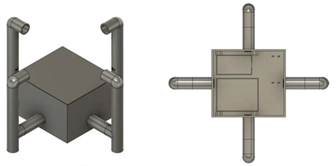
\includegraphics[width=\linewidth]{gambar/fig_anemometer_abdillah_skema}
	\caption{Alat Anemometer Ultrasonic di dalam ruangan \parencite{Abdillah2022}}
\end{figure}

\subsubsection{Rancang Bangun \emph{Thermal-Based Anemometer} dan Arah Angin untuk Aliran Udara Rendah}

\subsubsection{Sistem Pendeteksi Arah Angin Menggunakan \textit{Hot-Wire} Anemometer}

\subsubsection{Simulator Sensor Pengukur Jarak Berbasis Ultrasonic dan Infrared Menggunakan Kendali Jarak Jauh Dilengkapi Webcam Berbasis Web 
Interface}


\subsection{Angin}

% Contoh penggunaan referensi dari pustaka
Angin adalah udara yang bergerak dari daerah yang bertekanan udara tinggi (maksimum) ke daerah yang bertekanan udara rendah (minimum). Perbedaan 
tekanan udara di sebebabkan adanya perbedaan suhu udara. Apabila suhu udaranya tinggi maka tekanan udaranya minimum, sedangkan apabila suhu udaranya 
rendah maka tekanan udara maksimum. Alat utuk mengukur arah dan kecepatan angin adalah anemometer.

Faktor terjadinya Angin dalam proses terjadinya angin dipengaruhi oleh beberapa faktor yang menyebabkan angin muncul antara lain sebagai berikut. 
Gradien Barometris, adalah bilang yang menampilkan adanya perbedaan tekanan udara dari 2 isobar pada jarak 111 km. Dimana semakin besar gradien 
barometris, maka semakin cepat juga tiupan angin. Letak Tempat, adalah angin lebih cepat yang berada atau dekat di garis khatulistiwa, dari pada yang 
jauh dari khatulistiwa. Tinggi Tempat,Tinggi rendahnya tempat/lokasi dapat mempengaruhi karena semakin tinggi tempat tersebut, maka semakin kencang 
angin bertiup, dan sebaliknya, Hal ini dapat terjadi karena disebabkan oleh pengaruh gaya gesekan yang menghambat laju udara.

Di permukaan yang tidak merata seperti gunung, pohon dan tempat lainnya memberikan gaya gesekan yang besar. Waktu, Disiang hari angin bergerak lebih 
cepat dari pada di malam hari. Dalam klimatologi, angin memiliki dua fungsi dasar yaitu : Pemindahan panas baik dalam bentuk yang dapat diukur maupun 
yang tersimpan dari lintang rendah ke lintang yang lebih tinggi dan akan membuat setimbang neraca radiasi surya antara lintang rendah dan tinggi 
Pemindahan uap air yang dievaporasikan dari laut ke daratan dimana sebagian besar dikondensasikan untuk menyediakan kebutuhan air yang turun kembali 
sebagai hujan, kabut ataupun embun.fungsi angin secara umum juga adalah memindahkan uap air yang sudah terevaporasi dari laut ke daratan dan mengalamu 
kondensasi yang selanjutnya menjadi hujan.

\subsection{Anemometer}

Anemometer adalah alat untuk mengukur atau menentukan kecepatan angin. Anemometer merupakan salah satu instrument yang sering 
digunakan oleh Badan Meterologi Klimatologi dan Geofisika (BMKG). Kata anemometer berasal dari Bahasa Yunani anemos yang berarti angin, angin 
merupakan udara yang bergerak ke segala arah, angin bergerak dari suatu tempat menuju ke tempat yang lain. Anemometer ini pertama kali diperkenalkan 
oleh Leon Batista Alberti dari italia pada tahun 1450. Pada saat itu, model yang digunakan adalah Cup Anemometer.

\subsubsection{Cup Anemometer}
	Cup Anemometer adalah alat yang mempunyai baling-baling berbentuk setengah lingkaran dan menyerupai mangkok kecil. Ketika tertiup angin, mangkok 
  yang terdapat pada anemometer akan bergerak sesuai arah angin. Makin besar kecepatan angin meniup mangkok tersebut, makin cepat pula kecepatan 
  berputarnya piringan mangkok tersebut, makin cepat pula kecepatan berputarnya piringan mangkok. Dari jumlah putaran dalam satu detik maka dapat 
  diketahui kecepatananginnya. Didalam anemometer terdapat alat pencacah yang akan menghitung kecepatan angin.
	
	\subsubsection{Windmill Anemometer}
	
	Windmill Anemometer adalah anemometer di mana kincir angin didorong oleh aliran udara, dan rotasi ditransmisikan melalui gearing ke dial atau 
  mekanisme perekaman lainnya. Dalam beberapa instrumen, baling-baling dan dial yang berputar berada pada bidang yang sama yaitu, keduanya vertikal, 
  sementara di lain dial adalah horizontal. Dalam jenis kincir angin, pengoperasian pengukuran udara melibatkan pembacaan dial pada awal dan akhir 
  periode yang diukur. Instrumen kincir angin dapat dilengkapi dengan pegangan ekstensi, menyediakan bentuk kendali jarak jauh; digunakan untuk mengukur 
  kecepatan udara di tempat yang tidak dapat diakses.
	
	\subsubsection{Hot Wire/Thermal Anemometer}
	
	Thermal Anemometer atau dikenal juga dengan Hot Wire Anemometer adalah transduser termal yang banyak digunakan untuk mengukur kecepatan aliran udara 
  sesaat. Penggunaan anemometer hot wire memungkinkan kecepatan aliran sesaat dihitung dari pengukuran tegangan listrik [Kim et al., 2016]. Keuntungan 
  dari anemometer hot wire dikaitkan dengan resolusi spasial yang sangat tinggi dan karakteristik respons frekuensi yang sangat baik.
	
	\subsubsection{Ultrasonic Anemometer}
	
	Time of flight pulsa suara yang merambat di udara menyediakan metode lebih lanjut untuk merasakan kecepatan angin. Ultrasound dapat dengan mudah 
  dihasilkan dan dideteksi secara elektronik, dan digunakan untuk pengukuran tersebut. Dalam anemometer ultrasonik, waktu terbang yang diperlukan 
  pulsa ultrasound untuk bergerak maju dan mundur antara dua transduser tetap A dan B diukur. Karena responnya yang cepat, anemometer sonik sangat 
  cocok untuk pengukuran lapangan fluktuasi turbulen kecepatan angin, dan dalam beberapa arah secara bersamaan. vektor kecepatan tiga dimensi dapat 
  dihitung dengan beberapa pengolahan data dan identitas trigonometri (Harrison, 2014).
	
	Satu-satunya kelemahan signifikan dari instrumen ini adalah biaya dan pengelolaan volume data yang besar yang dapat dihasilkan dengan cepat. 
  Anemometer ultrasonik berfungsi untuk mengukur kecepatan dan arah angin. Didesain tanpa ada bagian yang bergerak, anemometer ultrasonik ini 
  diharapkan lebih handal, bebas perawatan, tahan lama, dan dapat beroperasi dalam kondisi cuaca yang ekstrim. Untuk tugas akhir ini dibatasi 
  sampai dengan pembuatan prototipe awal dan pembuktian bahwa sinyal ultrasonik akan berubah time of flight (ToF) nya ketika tranduser ultrasonik 
  dihembus oleh angin.

\subsection{Gelombang Ultrasonic}
Suara/akustik merupakan energi mekanik yang menyebar melalui suatu medium yang kontinu dan elastis dengan memampatkan dan menipiskan partikel 
sehingga mengubah susunannya. Ada dua tipe dasar dari gelombang akustik, yaitu gelombang longitudinal dan gelombang transversal. Pada gelombang 
longitudinal, gerak partikel pada suatu media akustik searah dengan perambatannya. Pada gelombang transversal,pergerakan partikelnya tegak lurus dengan arah rambatnya.

\begin{figure}[h!]
	\centering
	\includegraphics[width=0.7\linewidth]{"gambar/spektrum akustik"}
	\caption{Spektrum Akustik}
	\label{fig:spektrum-akustik}
\end{figure}

Gelombang ultrasonik merupakan gelombang mekanik longitudinal yang frekuensinya melampaui batas dengar telinga manusia (di atas 20 kHz), dan 
gelombangnya menyebar dalam medium baik padat, cair dan gas, yang disebabkan oleh osilasi bolak balik partikel pada titik kesetimbangan. 
Pada spektrum akustik seperti yang diperlihatkan oleh Gambar \ref{fig:spektrum-akustik}, gelombang ultrasonik berada pada sisi kanan spektrum akustik.

Pada frekuensi 10 kHz - 150 kHz, ultrasonik dipakai untuk komunikasi beberapa binatang seperti kelelawar dan lumba-lumba. Jika pada frekuensi ini 
dayanya ditingkatkan maka ultrasonic dapat dipakai untuk membantu proses pembersihan (cleaner) beberapa material misalkan perhiasan.Untuk aplikasi 
medical imaging dibutuhkan frekuensi dari 1 MHz sampai dengan 20 MHz misalkan seperti yang dipakai untuk ultrasonografi (USG).

\subsection{Perambatan Gelombang Ultrasonic}

Gelombang ultrasonik yang dihasilkan oleh transduser dapat berupa sinyal pulsa atau sinyal kontinu, tergantung pada tegangan yang diinputkan pada 
transduser. Mode apa yang akan dipakai tergantung pada metode tes yang akan digunakan. 

Karakteristik gelombang ultrasonik yang melalui medium mengakibatkan getaran partikel dengan medium amplitudo sejajar dengan arah rambat secara 
longitudinal sehingga menyebabkan partikel medium membentuk rapatan (strain) dan tegangan (stress). Proses kontinu yang menyebabkan terjadinya rapatan 
dan regangan di dalam medium disebabkan oleh getaran partikel secara periodic selama gelombang ultrasonik melaluinya (Resnick et al., 1992).

Gelombang ultrasonik di dalam material dapat merambat dengan tiga macam pola gelombang yang sering digunakan, yaitu gelombang longitudinal, 
gelombang transversal, gelombang permukaan atau Rayleigh waves. 

Gelombang longitudinal merupakan gelombang yang paling sering digunakan untuk pengujian ultrasonik. Kelebihan gelombang ini adalah kemampuannya 
yang dapat merambat di dalam zat cair dan gas, sama baiknya seperti pada material solid. Mekanisme gelombang ini adalah perambatannya sejajar 
dengan arah gerakan atom yang digetarkan.

\begin{figure}
	\centering
	\includegraphics[width=0.7\linewidth]{"gambar/pergerakan partikel"}
	\caption{Pergerakan partikel akibat gelombang longitudinal (kiri) dan gelombang transversal (kanan) (k arah pergerakan gelombang, l jarak 
  antara atom yang bersebelahan) (Still, 2009)}
	\label{fig:pergerakan-partikel}
\end{figure}

Gelombang transversal merupakan jenis gelombang yang juga sering digunakan, tetapi tidak seperti gelombang longitudinal, gelombang ini sulit 
merambat dalam zat cair dan gas, karena karakternya yang kurang elastis dan dibutuhkan gaya yang kuat pada partikel untuk berosilasi. Gelombang 
ini dapat terjadi apabila gelombang ultrasonik merambat pada arah yang tegak lurus, dengan vibrasi yang bergerak ke atas dan ke bawah, pada arah 
dan bidang gerakan atom yang digetarkan. Ilustrasi dari gelombang ini secara skematis ditunjukkan pada Gambar \ref{fig:pergerakan-partikel} yang 
menunjukkan pergerakan partikel berpengaruh terhada perambatan dari gelombang longitudinal dan transversal.

\subsection{Sensor Jarak Ultrasonik}

Sensor ultrasonik adalah sebuah sensor yang mengubah besaran fisis (bunyi) menjadi besaran listrik. Sensor ultrasonik ini menggunakan ultrasound, 
dimana ia menggunakan frekuensi suara yang sangat tinggi diatas batas pendengaran manusia. Rata-rata manusia mempunyai batas pendengaran sekitar 20 
KHz, sehingga sensor menggunakan batas diatas pendengaran manusia. Pulsa dari gelombang suara ultrasonik dikirim dari transducer dan kemudian diambil 
lagi menggunakan transducer yang sama ketika memantul ke sebuah objek. Dari kalkulasi waktu yang digunakan untuk suatu pulsa dapat kembali ditunjukkan 
pada Gambar 2.x. Kecepatan pengiriman gelombang suara di udara kering pada suhu 20 Celsius adalah 340 m/s.

\begin{figure}[h!]
	\centering
	\includegraphics[width=0.7\linewidth]{"gambar/diagram kerja sensor ultrasonic"}
	\caption{Prinsip jarak sonar atau radar pengukuran.}
	\label{fig:diagram-kerja-sensor-ultrasonic}
\end{figure}

Pada sensor ini gelombang ultrasonik dibangkitkan melalui sebuah benda yang disebut piezoelektrik. Piezoelektrik ini akan menghasilkan gelombang 
ultrasonik dengan frekuensi 40 kHz. Sensor ultrasonik secara umum digunakan untuk suatu pengungkapan tak sentuh yang beragam seperti aplikasi 
pengukuran jarak. Bentuk fisik dari sensor ultrasonik seperti pada Gambar \ref{fig:sensor-ultrasonic}

\begin{figure}[h!]
	\centering
	\includegraphics[width=0.7\linewidth]{"gambar/sensor ultrasonic"}
	\caption{Modul HC-SR04.}
	\label{fig:sensor-ultrasonic}
\end{figure}

Modul HC-SR04 memiliki 4 kaki pin yaitu pin Vcc, pin Trig, pin Echo, dan pin GND dengan fungsi yang berbeda-beda. Pada pin Vcc berfungsi 
sebagai pemberi tegangan ke sensor ultrasonik. Pin Trig atau sama dengan pin trigger adalah pin yang berfungsi sebagai pemicu untuk memantulkan 
sinyal pantul. Sedangkan pada pin echo berfungsi sebagai pin receiver atau pin penerima dari sinyal pantul yang dihasilkan oleh pin trigger. 
Dan pin GND atau sama dengan pin ground berfungsi sebagai pin penetral.

\begin{table}
	\caption{Spesifikasi HC-SR04}
	\centering
	\begin{tabular}{|c|c|}
		\hline
		Working Voltage & DC 5V \\
		\hline
		Working Current & 15mA \\
		\hline
		Working Frequency & 40 KHz \\
		\hline
		Max Range & 4m \\
		\hline
		Min Range & 2cm \\
		\hline
		Measuring Angle & 15 \\
		\hline
		Trigger Input Signal &  TTL Pulse \\
		\hline
		Echo Output Signal & Input TTL lever signal and the range in proportion \\
		\hline
		Dimension & 45*20*15 mm \\
		\hline
	\end{tabular}
\end{table}

Karena sistem kerja sensor jarak ultrasonik ini adalah dengan menggunakan cara menembakkan gelombang ke objek dan menunggu 
pantulannya maka membutuhkan waktu tempuhnya dua kali, sehingga untuk mengetahui jarak sebenarnya harus dibagi dua. Dimana 
jarak setengah awal adalah waktu gelombang ditembakkan dan mengenai obyek, jarak setengah berikutnya adalah pantulan 
gelombang dari obyek yang kembali ke receiver. Jarak yang diukur menggunakan rumus seperti pada Persamaan 2.1.

\begin{equation}\label{rumus jarak}
	 S= V * t : 2
\end{equation}

Dimana S adalah jarak antara pemancar dan penerima dalam satuan meter (m), V adalah kecepatan suara yaitu 340 m/s, t adalah 
waktu tempuh dalam satuan detik (s).

\subsection{Time of Flight (ToF)}

Time of Flight adalah pengukuran waktu yang diperlukan oleh suatu benda, partikel atau gelombang (baik akustik, elektromagnetik, 
dll.) untuk menempuh jarak melalui media. Informasi ini kemudian dapat digunakan untuk mengukur kecepatan atau panjang lintasan, 
atau sebagai cara untuk mempelajari tentang sifat partikel atau medium (seperti komposisi atau laju aliran). 

Miguel Perez del Valle, Jose Antonio Urbano Castelan, Yasuhiro Matsumoto, dan Rau’l Cortes Mateos dalam penelitiannya menyatakan 
Kecepatan rambat suara di udara dipengaruhi oleh komponen kecepatan aliran udara(angin). Jika angin mengalir dalam arah rambat 
suara maka akan meningkatkan kecepatan rambat suara, sedangkan jika angin mengalir berlawanan dengan arah rambat suara, maka 
kecepatan rambat suara akan menurun (del Valle et al., 2007).

\subsection{Raspberry Pi Pico W}



  % Konten metodologi
  \section{METODOLOGI}

% Ubah konten-konten berikut sesuai dengan isi dari metodologi

\subsection{Metode yang digunakan}

\begin{figure}[h!]
	\centering
	\includegraphics[width=0.5\linewidth]{"gambar/Flowchart penelitian.drawio"}
	\caption{Flowchart Penelitian}
	\label{fig:flowchart-penelitian}
\end{figure}

Pada Tugas Akhir ini, garis besar alur Tugas Akhir dapat dilihat pada Gambar \ref*{fig:flowchart-penelitian}. Berikut penjelasan
dari tiap tahapan pada Gambar \ref{fig:flowchart-penelitian}.

\begin{enumerate}
  \item Studi Literatur
  
  Studi literatur adalah metode awal yang dilakukan guna mencari materi-materi penunjang dari pengembangan anemometer ultrasonic 
  dalam ruangan berbasis Raspberry Pi Pico. Studi literatur ini dilakukan dengan mempelajari dan menganalisis dari rancang bangun 
  anemometer yang telah dibuat sebelumnya. Baik berupa penggunaan sensor, aktuator, maupun metode penelitian sebagai bahan penunjang 
  tambahan dari gagasan yang akan direalisasikan. Dalam pencarian studi literatur ini dilakukan referensi dari buku, jurnal penelitian, 
  ataupun artikel ilmiah yang berkaitan dengan gagasan yang dibawa. Data yang sudah terkumpul dari studi literatur sebelumnya dikumpulkan
  dan diolah untuk penunjang gagasan yang direalisasikan.

  \item Persiapan Rancang Bangun Anemometer Ultrasonic

  \begin{figure}[h!]
    \centering
    \includegraphics[width=0.4\linewidth]{"gambar/Blok diagram anemometer ultrasonic"}
    \caption{Blok Diagram Sistem}
    \label{fig:blok-diagram-anemometer-ultrasonic}
  \end{figure}

  Model sistem yang digunakan dapat dilihat pada  gambar \ref{fig:blok-diagram-anemometer-ultrasonic}. Prototipe anemometer ultrasonic dalam ruangan berbasis 
  Raspberry Pi Pico ini akan dilengkapi dengan Website yang dapat menampilkan hasil data yang diperoleh alat secara real-time. Pengujian prototipe ini akan dilakukan 
  dengan menghitung kecepatan angin pada saat kondisi normal dengan jarak konstan, kemudian hasilnya akan dibandingkan dengan anemometer hot-wire komersial. 

  \item Perancangan Perangkat komersial
  
  Pada penelitian kali ini akan dilakukan pembuatan desain alat menggunakan aplikasi Fusion 360, dimana hasilnya akan dicetak menggunakan printer 3D. Selain desain alat, terdapat komponen
  penting lainnya seperti sensor Ultrasonic, sensor suhu, penggaris, dan LCD untuk menampilkan informasi. Setelah seluruh komponen dijadikan prototipe, maka akan dilanjutkan ke tahap kalibrasi

  \item Kalibrasi Sensor Ultrasonic

\begin{figure}[h!]
	\centering
	\includegraphics[width=0.7\linewidth]{"gambar/Diagram blok pengukuran kecepatan angin.drawio"}
	\caption{Blok Diagram Perhitungan Kecepatan Angin}
	\label{fig:diagram-blok-pengukuran-kecepatan-angin}
\end{figure}

  Untuk menemukan konversi dari pembacaan sensor yang tepat. Dilakukan beberapa percobaan dengan berbagai kondisi dan variabel untuk menentukan rumus yang tepat untuk digunakan sebagai rumus umum.
  Adapun diagram blok sistem pengukuran kecepatan angin pada alat ini dapat dilihat pada Gambar \ref{fig:diagram-blok-pengukuran-kecepatan-angin}.

  \item Perancangan Perangkat Lunak
  
  Pada penelitian kali ini dibutuhkan perancangan perangkat lunak untuk menghubungkan antara hasil pembacaan sensor ultrasonic dengan website melalui jaringan internet.

  \item Pembuatan Website untuk menampilkan data alat
  
  Secara garis besar, website akan menampilkan kecepatan angin dari prototipe alat secara real-time.
  
  \item Koneksi Anemometer ultrasonic dengan Website
  
  Pada tahapan ini, akan dilakukan penghubungan antara perangkat keras dengan perangkat lunak sehingga prototipe alat dapat terhubung dengan internet dan data yang diperoleh dapat dilihat melalui 
  website. Jika semua sudah terkoneksi dengan benar maka akan dilanjutkan pada tahap pengujian.

  \item Pengujian alat dan pengambilan data
  
  Pada tahap pengujian akan dilakukan pengujian pengukuran kecepatan angin. Pengujian alat ini menggunakan metode perubahan variabel kecepatan angin kemudian dilakukan perbandingan 
  antara hasil pengukuran dari alat prototipe dengan hasil pengukuran dari anemometer Hot-wire komersial.
  \item Penarikan kesimpulan
  
  Berdasarkan data yang diperoleh dari tahap pengujian, dilakukan analisa dan didapatkan kesimpulan yang menjawab dari perumusan masalah yang terdapat pada bab I. 
\end{enumerate}

\subsection{Bahan dan peralatan yang digunakan}

Untuk Alat dan bahan penunjang penelitian Tugas Akhir ini adalah sebagai berikut:
\begin{enumerate}
  \item Raspberry Pi Pico W
  
  Raspberry Pi Pico W adalah sebuah board minimum sistem mikrokontroller yang berbasis chip RP2040 didalamnya. 
  Alat ini digunakan untuk membaca data dari sensor ultrasonic dan memproses data hasil bacaan sensor. Selain itu, 
  mikrokontroller ini sudah memiliki modul wifi didalamnya sehingga dapat mengirimkan data langsung ke server database 
  melalui jaringan wifi internet.

  \item Modul Ultrasonic US-100
  
  Merupakan sensor ultrasonic yang umumnya digunakan sebagai pengukur jarak, namun pada penelitian ini digunakan sebagia
  pengukur kecepatan angin. Modul sensor ini terdiri dari sepasang transducer ultrasonic, salah satu bagian berfungsi sebagai 
  transmitter yang mengubah sinyal elektrik menjadi sinyal pulsa gelombang suara ultrasonic dengan frekuensi 40KHz., dan bagian lainnya 
  berfungsi sebagai receiver yang berfungsi menerima sinyal gelombang ultrasonic.
  \item Sensor Suhu
  
  Sensor suhu digunakan untuk mengetahui kondisi temperatur sekitar dari alat prototipe yang dibangun. Hal ini berguna sebagai variabel 
  pendukung dikarenakan salah satu parameter dalam kecepatan angin adalah suhu udara sekitar.
\end{enumerate}

\subsection{Urutan pelaksanaan penelitian}

Berikut jadwal pelaksanaan kegiatan Tugas Akhir selama 16 minggu, dapat dilihat pada tabel \ref{tbl:timeline}.
% Ubah tabel berikut sesuai dengan isi dari rencana kerja
\newcommand{\w}{}
\newcommand{\G}{\cellcolor{gray}}
\begin{table}[h!]
  \begin{tabular}{|p{3.5cm}|c|c|c|c|c|c|c|c|c|c|c|c|c|c|c|c|}

    \hline
    \multirow{2}{*}{Kegiatan} & \multicolumn{16}{|c|}{Minggu} \\
    \cline{2-17} &
    1 & 2 & 3 & 4 & 5 & 6 & 7 & 8 & 9 & 10 & 11 & 12 & 13 & 14 & 15 & 16 \\
    \hline

    % Gunakan \G untuk mengisi sel dan \w untuk mengosongkan sel
    Studi Literatur &
    \G & \w & \w & \w & \w & \w & \w & \w & \w & \w & \w & \w & \w & \w & \w & \w \\
    \hline

    Persiapan Alat dan Bahan &
    \w & \G & \G & \w & \w & \w & \w & \w & \w & \w & \w & \w & \w & \w & \w & \w \\
    \hline

    Perancangan Perangkat Keras &
    \w & \w & \w & \G & \G & \w & \w & \w & \w & \w & \w & \w & \w & \w & \w & \w \\
    \hline

    Kalibrasi Sensor &
    \w & \w & \w & \w & \w & \G & \G & \w & \w & \w & \w & \w & \w & \w & \w & \w \\
    \hline

    Perancangan Perangkat Lunak &
    \w & \w & \w & \w & \w & \w & \w & \G & \G & \w & \w & \w & \w & \w & \w & \w \\
    \hline

    Pembuatan Website &
    \w & \w & \w & \w & \w & \w & \w & \w & \w & \G & \G & \w & \w & \w & \w & \w \\
    \hline

    Koneksi Antara Alat dengan Website &
    \w & \w & \w & \w & \w & \w & \w & \w & \w & \w & \w & \G & \w & \w & \w & \w \\
    \hline

    Pengujian Alat &
    \w & \w & \w & \w & \w & \w & \w & \w & \w & \w & \w & \w & \G & \G & \w & \w \\
    \hline

    Penarikan Kesimpulan &
    \w & \w & \w & \w & \w & \w & \w & \w & \w & \w & \w & \w & \w & \w & \G & \G \\
    \hline

  \end{tabular}
  \captionof{table}{Tabel timeline}
  \label{tbl:timeline}
\end{table}



  % Konten lainnya
  \section{HASIL YANG DIHARAPKAN}

\subsection{Hasil yang Diharapkan dari Penelitian}

Dari penelitian yang akan dilakukan, diharapkan mampu menambah wawasan penulis dalam merancang alat anemometer ultrasonic serta
menambahkan penelitian mengenai Raspberry Pi Pico yang saat ini masih jarang ditemukan di kampus ITS.

\subsection{Hasil Pendahuluan}

Telah dilakukan percobaan untuk menganalisa
sinyal pulsa yang diterima dari sensor Ultrasonic US-100. Percobaan dilakukan menggunakan alat Logic Analyser dari Saleae. Kemudian hasil dari logic analyser dibandingkan dengan output yang muncul pada 
serial Raspberry Pi Pico.

\begin{figure}[h!]
	\centering
	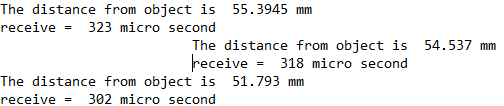
\includegraphics[width=0.7\linewidth]{gambar/serial5cm}
	\caption{Output Serial pada jarak 5cm}
	\label{fig:serial5cm}
\end{figure}

Pada percobaan pertama dilakukan pengukuran pada jarak 5 cm. Hasil dari sensor ultrasonic pada output 
serial dapat dilihat pada gambar \ref{fig:serial5cm}. Hasilnya berupa jarak yang terukur 54.537 mm atau 5.46 cm dengan \textit{ToF} 318 mikrosekon. Berikutnya pada logic analyser didapatkan pengukuran 
delta waktu sebesar 318.563 mikrosekon yang dapat dilihat pada gambar \ref{fig:logic5cm}.

\begin{figure}[h!]
	\centering
	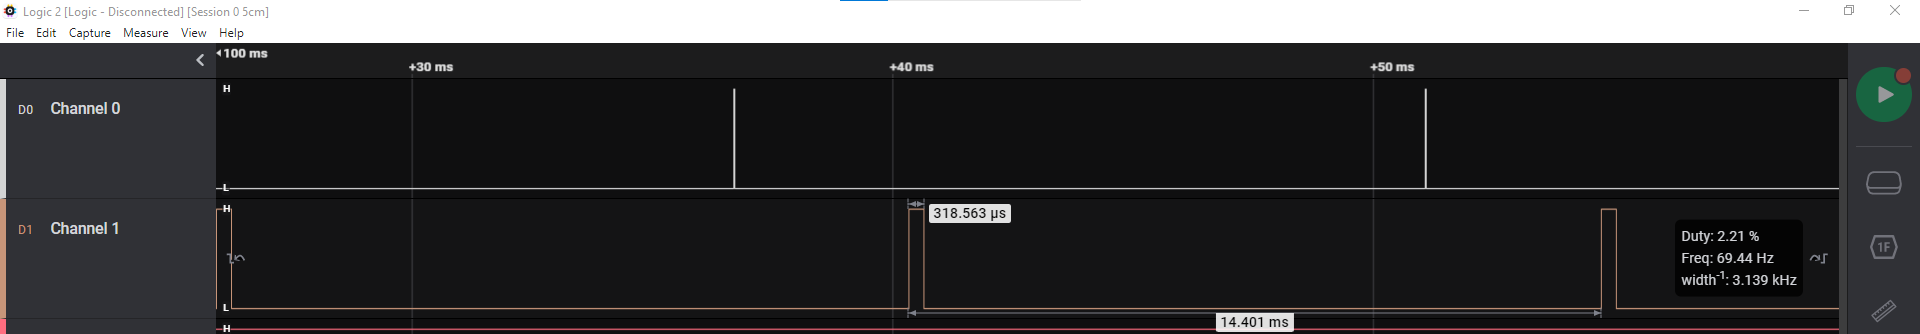
\includegraphics[width=\linewidth]{gambar/logic5cm}
	\caption{Output Sinyal Digital pada jarak 5cm}
	\label{fig:logic5cm}
\end{figure}

\begin{figure}[h!]
	\centering
	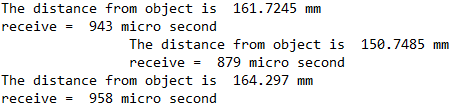
\includegraphics[width=0.7\linewidth]{gambar/serial15cm}
	\caption{}
	\label{fig:serial15cm}
\end{figure}

Pada percobaan kedua dilakukan pengukuran pada jarak 15 cm. Hasil dari sensor ultrasonic pada output 
serial dapat dilihat pada gambar \ref{fig:serial15cm}. Hasilnya berupa jarak yang terukur 150.7485 mm atau 15.75 cm dengan \textit{ToF} 879 mikrosekon. Berikutnya pada logic analyser didapatkan pengukuran 
delta waktu sebesar 879.625 mikrosekon yang dapat dilihat pada gambar \ref{fig:logic15cm}.

\begin{figure}[h!]
	\centering
	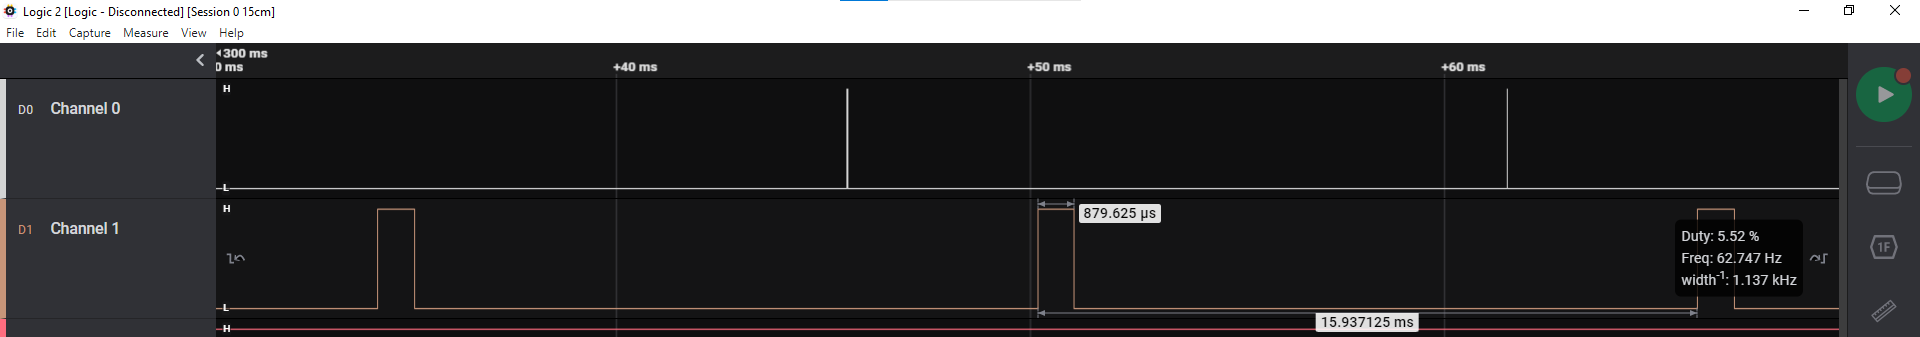
\includegraphics[width=\linewidth]{gambar/logic15cm}
	\caption{}
	\label{fig:logic15cm}
\end{figure}

\begin{figure}[h!]
	\centering
	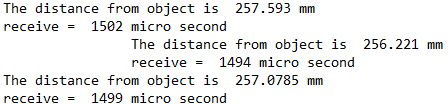
\includegraphics[width=0.7\linewidth]{gambar/serial25cm}
	\caption{}
	\label{fig:serial25cm}
\end{figure}

Pada percobaan ketiga dilakukan pengukuran pada jarak 25 cm. Hasil dari sensor ultrasonic pada output 
serial dapat dilihat pada gambar \ref{fig:serial25cm}. Hasilnya berupa jarak yang terukur 256.221 mm atau 25.62 cm dengan \textit{ToF} 1494 mikrosekon. Berikutnya pada logic analyser didapatkan pengukuran 
delta waktu sebesar 1494.625 mikrosekon atau 1.494 milisekon yang dapat dilihat pada gambar \ref{fig:logic25cm}.

\begin{figure}[h!]
	\centering
	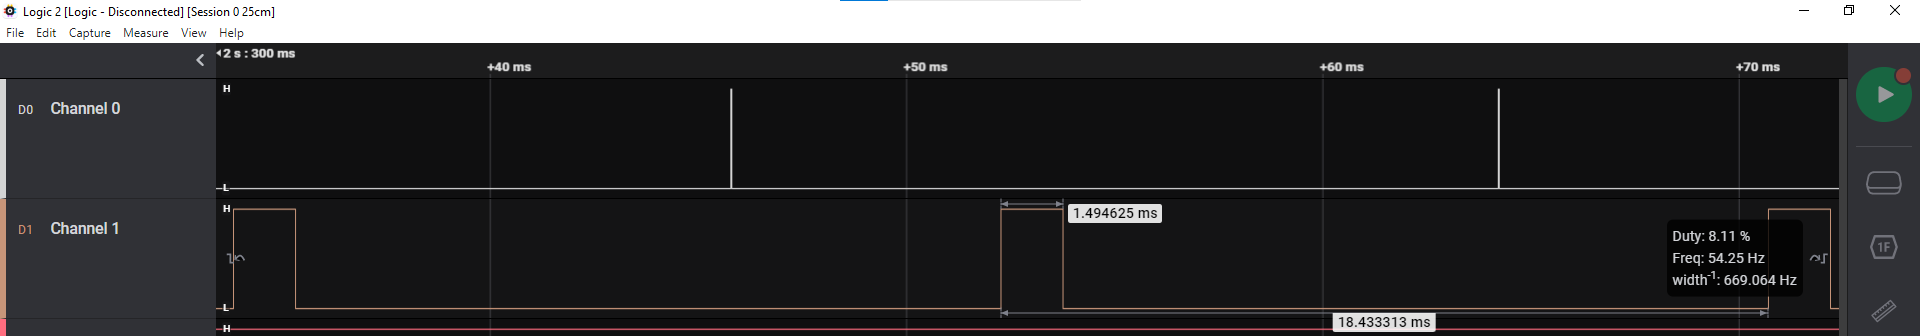
\includegraphics[width=\linewidth]{gambar/logic25cm}
	\caption{}
	\label{fig:logic25cm}
\end{figure}



  % Daftar pustaka
  \section{DAFTAR PUSTAKA}
  \renewcommand\refname{}
  \vspace{2ex}
  \renewcommand{\bibname}{}
  \begingroup
    \def\chapter*#1{}
    \printbibliography
  \endgroup


\end{document}

